\cleardoublepage

\section{项目实施方案}

\subsection{软件需求分析}

本项目的目标是实现一个高效的工业场景渲染系统,以下是针对关键需求的分析:

\par (1)\textbf{工业模型导入及数据预处理要求:}  
系统需要支持包含千万级多边形的工业模型导入,并确保数据预处理与加载过程在 1 小时内完成。同时,内存占用不得超过 24GB。为此,系统应具备高效的流式加载机制以及对大规模模型的分布式存储和处理能力,以确保能够在有限时间内完成复杂数据的处理和加载。

\par (2)\textbf{运行时性能要求:}  
在运行时,系统显存占用不超过 8GB,且渲染帧率需稳定在 30FPS 左右。此外,系统应保持较高的画面质量,确保渲染结果与原始模型的视觉差异控制在可接受范围内。这要求系统具备先进的 LOD 管理与流式加载策略,通过合理的显存管理与优化技术,保证高效渲染同时不超过显存限制。

\par (3)\textbf{与现有技术对比:}  
在帧率、显存占用、内存占用、预处理时间以及画面保真度等关键性能指标上,本项目应至少达到与虚幻引擎 Nanite 相当的水平,并在部分方面实现超越。例如,优化流式加载与 LOD 策略,使得系统能够在相同硬件上实现更高效的运行,同时降低预处理时间和显存占用。

\par (4)\textbf{鲁棒性与适应性要求:}  
系统需要具有较强的鲁棒性,能够适应不同类型的工业场景及 CAD 模型,并能根据不同硬件配置进行优化。为此,系统应具备灵活的硬件适配能力,并支持动态调整渲染管线与内存使用策略,确保在不同硬件环境下都能达到预期性能。

\subsection{项目整体架构}

\par 本项目的整体流程可分为预处理阶段与运行时阶段,如\autoref{fig:流程}所示。其中,预处理阶段主要负责将原始模型从磁盘加载至内存,并对其进行结构化处理。具体包括:将模型划分为多个簇(cluster/meshlet)、为各子模型生成多层次细节(LOD),并将处理后的数据组织成便于流式加载的格式。这些经过预处理的场景信息将被缓存在 CPU 内存中,为运行时的按需加载提供数据支撑。

\par 在运行时阶段,主要包括几何处理模块与流式加载模块两个核心部分。几何模块负责生成 G-Buffer\cite{lauritzen2010},为后续的光照计算等渲染阶段提供基础几何信息。在任务着色器(Task Shader)中,不仅执行 LOD 选择与可见性剔除,还根据结果评估当前视角所需的几何数据,进而为流式加载模块提供调度指引。流式加载模块则依据几何模块的请求,将相应的场景数据按需加载至 GPU 内存,实现高效的数据管理与实时渲染支持。渲染管线的其余部分(如绘制指令预处理、光照与后处理等)则由原有自研引擎模块提供支持。

\begin{figure}[htbp]
    \centering
    \includegraphics[width=\linewidth]{流程.jpg}
    \caption{\label{fig:流程}项目流程图}
\end{figure}

\par 综上所述,本项目在原有引擎渲染管线的基础上,主要负责对几何模块进行修改,新增流式加载模块,并在预处理阶段实现了模型划分成簇与生成 LOD 的功能。通过这些改进,原渲染管线的性能得到了显著优化,帧率明显提升,显存占用有所降低,同时保持了良好的画面保真度。

\section{基于簇的 GPU 驱动渲染管线}

\subsection{引言}

GPU 驱动的渲染管线是一种通过 GPU 完成大部分渲染任务的渲染架构,与传统的 CPU 驱动渲染管线相比,GPU 驱动渲染管线能够显著提高渲染效率,尤其在处理复杂或大规模场景时。其核心思想是将大量渲染计算和数据处理任务交给 GPU 执行,充分利用 GPU 强大的并行计算能力,从而加速渲染过程。

在传统的 CPU 驱动渲染管线中,CPU 通常承担着场景遍历、物体剔除、LOD 管理等任务,而 GPU 主要负责图形的绘制和光照计算等工作。然而,随着图形渲染需求的提升,CPU 驱动渲染管线的性能瓶颈逐渐显现,特别是在处理大规模场景时,CPU 的计算负担较重,出现渲染性能下降等问题\cite{Tian2024}。

而在 GPU 驱动的渲染管线中,许多原本由 CPU 执行的任务(如剔除计算、LOD 选择等)都转移到 GPU 上,这样可以减少 CPU 的负担,使得 GPU 能够在更高效的并行计算模式下进行工作。

本项目除了流式加载模块中涉及到 CPU 与 GPU 之间的通信外,其余操作均在 GPU 上实现。与此同时,本项目引入了由任务着色器和网格着色器组成的新型渲染管线,代替了传统的计算着色器(Compute Shader)、顶点着色器(Vertex Shader)和几何着色器(Geometry Shader)的组合。通过将渲染单元组织为簇(Meshlet)并以簇为单位进行处理,进一步提升了渲染性能和灵活性\cite{Czubala2024}。

\subsection{基于簇的渲染}

基于簇的渲染最早由育碧(Ubisoft)在游戏《刺客信条:大革命》(Assassin's Creed Unity)中提出\cite{Ubisoft2015}。该方法将最小的剔除单元从传统的实例(instance)替换为簇,每个簇包含多个三角形,一个实例可以包含多个簇。通过这种更加细粒度的剔除方式,渲染引擎能够根据簇的可见性进行精确剔除,避免了传统基于实例的剔除方法中对大范围不必要的几何数据进行处理。对于复杂模型,这种做法能减少需要绘制的几何体数量,从而显著降低渲染管线中的计算负担。

本项目在预处理阶段实现了簇的划分,并设计了基于簇的渲染管线,有效提升了运行时的渲染性能。

\subsubsection{簇的划分} \label{subsubsec:cluster division}

簇的划分是本项目预处理阶段的关键步骤之一,本项目使用了第三方库 MeshOptimizer 来实现这一过程\cite{meshoptimizer}。MeshOptimizer 是一个高效的网格优化库,提供了各种优化算法,可以有效地对网格进行简化和组织,从而提高 GPU 渲染的性能。在具体实现中,本项目规定每个簇最多由 64 个顶点 和 124 个三角形组成。这样的划分方式有助于平衡簇的大小和渲染效率\cite{Kubisch2018}。

\subsubsection{基于簇的剔除} \label{subsubsec:cluster culling}

基于簇的剔除是在任务着色器中进行的,剔除可分为视锥剔除(Frustum Culling)和圆锥剔除(Cone Culling)。

其中,视锥剔除是指通过测试模型的包围球与视锥体的关系,判断模型是否位于当前视锥内。每一个簇都拥有自己的包围球(Bounding Sphere),可以通过测试包围球与每个视锥平面的关系,来判断该簇是否可能在相机的视锥范围内。如果包围球完全在视锥体外,则该簇可以被剔除,避免不必要的渲染计算。

而圆锥剔除则是通过将簇的可见性表达为一个圆锥形状来进行判断,圆锥的范围包含了簇的所有法线方向。具体而言,如果相机的视角方向与圆锥范围内的所有法线方向的点积均为负数,则说明该簇背对着相机,可以整体剔除,不需要渲染。为了便于进行圆锥剔除,MeshOptimizer 库在预处理阶段会为每个簇生成相应的圆锥信息,包括圆锥的顶点、主轴方向和定角等参数,这些信息可以直接用于运行时的剔除操作,大大提高了渲染效率。

\subsubsection{基于簇的网格着色器渲染管线}

网格着色器是基于簇的渲染工作流程中的关键步骤之一。在这一阶段,经过任务着色器剔除后的簇将被并行处理,网格着色器负责对簇进行顶点变换、图元组装等操作。每个簇包含多个顶点和图元,网格着色器能够高效地并行处理多个簇,显著减少传统渲染管线中的处理开销\cite{Santerre2020}。

经过网格着色器处理后,簇将会被传递给片段着色器,这是工作流程的最后一步。片段着色器根据顶点的颜色、法线、纹理坐标等信息,计算每个像素的位置、法线和颜色等,用于后续的光照计算。网格着色器与片段着色器的协作,使渲染管线在处理大规模网格时保持高效且灵活。

\subsection{测试分析报告}

本项目实现了簇的可视化功能,并在多个场景中进行了测试,如 \autoref{fig:Meshlet} 所示。可以看出,簇划分结果较为规整,能够较好地贴合几何结构,且不同场景下的可视化效果均展现出了良好的适应性和一致性。这为后续的基于簇的剔除与 LOD 管理提供了直观支撑。

% \begin{figure}[htbp]
%     \centering
%     \includegraphics[width=\linewidth]{Meshlet.png}
%     \caption{\label{fig:Meshlet}簇的可视化效果图}
% \end{figure}

\begin{figure*}[htbp]
    \centering

    \begin{subfigure}[b]{0.48\linewidth}
        \centering
        \includegraphics[width=\linewidth]{Meshlet.png}
        \caption{Sponza 场景}
    \end{subfigure}
    \hfill
    \begin{subfigure}[b]{0.48\linewidth}
        \centering
        \includegraphics[width=\linewidth]{factory_meshlet.png}
        \caption{Factory 场景}
    \end{subfigure}

    \caption{簇的可视化效果图}
    \vspace{-0.2cm}
    \label{fig:Meshlet}
\end{figure*}

与此同时,本项目对 Factory 场景设置了固定相机轨迹进行测试,测量了不同剔除策略下的平均帧时间,以及 GPU 在裁剪阶段丢弃的平均图元数量。GPU 在裁剪阶段丢弃的图元数量越多,意味着处理了更多无效的几何数据,从而浪费了带宽和计算资源。具体测试结果见\autoref{tab:culling}。

\begin{table}[H]
    \caption{\label{tab:culling}不同剔除策略下的渲染性能测试结果}
    \begin{tabularx}{\linewidth}{|c|X<{\centering}|c|}
        \hline
        剔除策略 & GPU 在裁剪阶段丢弃的图元数 & 帧时间 \\ \hline
        不使用剔除 & 40713.9k & 240.7ms \\ \hline
        使用实例级剔除 & 40350.5k & 233.5ms \\ \hline
        使用视锥剔除 & 28557.5k & 147.9ms \\ \hline
        使用圆锥剔除 & 39249.1k & 230.7ms \\ \hline
        同时使用视锥剔除和圆锥剔除 & 27575.3k & 142.7ms \\ \hline
    \end{tabularx}
\end{table}

从表中数据可以看出,实例级的剔除对于工业大场景的性能提升有限,而基于簇的视锥剔除和圆锥剔除能够有效减少绘制三角形的数量。二者相结合的基于簇的剔除策略显著提升了渲染帧率,证明了基于簇的渲染方法在提高渲染效率方面的有效性。

\section{LOD机制}

\subsection{引言}

LOD(Level of Detail,细节层次)是一种通过根据物体与视点的距离调整其细节程度的技术。当物体距离视点较远时,可以使用较低的细节模型,而当物体接近视点时,则使用更高的细节模型。这种技术能显著减少不必要的计算量,提高渲染性能\cite{Deng2017}。而在本项目中,LOD不仅用于提高渲染性能,还与流式加载结合,进一步降低了显存占用。通过按需加载不同细节层次的模型,能够在保证画面质量的同时,优化显存资源的使用。

\subsection{LOD生成} \label{subsec:LOD generation}

LOD 生成部分参考了 Nanite 的核心思想,采用基于网格简化的 LOD 生成方法\cite{Jensen2023},整体过程大致可以分为以下几步\cite{Xavier2024}:

\newcommand{\stepref}[1]{\textbf{Step~\ref{#1}}}

\begin{enumerate}
    \item 将初始模型划分为簇;
    \item 根据簇之间的连接性,将簇组织成簇组(cluster group),每个簇组最多包含 16 个簇;
    \item 对每个簇组进行独立简化,确保每个簇组的边界完整,从而避免不同 LOD 之间出现裂缝;
    \item 将简化后的簇组重新划分为新的簇;
    \item 如果新的簇数量仍然过多,则返回步骤 2 进行进一步简化;否则,结束生成过程。
\end{enumerate}

其中,步骤 1 已经在\ref{subsubsec:cluster division}节中,通过使用 MeshOptimizer 库得到了有效解决。步骤 4 也可以采用类似的方法来处理。

在步骤 2 中,本项目将已生成的簇进一步划分为若干簇组。理想情况下,簇组之间的共享边应尽可能少,以最大程度减少后续步骤中因跨组操作而需锁定的顶点数量。该问题可等效视为串行图划分(Serial Graph Partitioning)问题,该问题可采用 METIS 等图划分库进行高效求解\cite{METIS}。

划分完成后,对于每个簇组,将继续使用 MeshOptimizer 库进行简化,即步骤 3。简化结束后,MeshOptimizer 库会返回一个误差值,用以表示简化后的网格与原网格的相对误差。该误差值将在 \ref{subsec:run-time lod select} 节中用于运行时的 LOD 选择。

为了确保简化过程能够顺利进行,还需要将距离较近的顶点进行合并。这是因为,在处理拓扑不一致或具有多个接缝的网格时,简化器可能会“卡住”,无法顺利完成简化任务。顶点合并能够有效推动简化器去除更多的三角形,从而促进简化过程。

为了高效地查找每个顶点的最近邻,本项目采用了 K-D 树进行管理\cite{bentley1975}。K-D 树的构建时间复杂度为 $O(N\log N)$,查询时间复杂度为 $O(\log N)$,具有较高的效率。

此外,为了避免顶点合并后簇组的视觉误差过大,本项目在顶点合并时不仅考虑顶点之间在空间中的距离,还将纹理坐标、法向量等其他因素纳入考虑范围。

为降低预处理开销,本项目引入 oneTBB 库对 LOD 生成过程进行多线程加速,从而提升了在大型工业场景下的处理效率与整体性能\cite{oneTBB}。

在完成以上所有步骤后,不同 LOD 等级的簇将构成一个有向无环图(DAG),如\autoref{fig:DAG}所示\cite{WangXi2022}。该图中,每个节点表示一个簇,且每个节点可能有多个父节点。被矩形框住的节点表示一个簇组。假设节点 A 和 B 是节点 C、D、E 和 F 的父节点,那么就意味着节点 A 和 B 是由簇组 C、D、E 和 F 中的簇简化得到的。在随后的运行时阶段,本项目将基于该有向无环图来进行 LOD 选择。

\begin{figure}[ht]
    \centering
    \includegraphics[width=\linewidth]{DAG.png}
    \caption{\label{fig:DAG}LOD的DAG示意图}
\end{figure}

\subsection{运行时 LOD 选择} \label{subsec:run-time lod select}

\par 对于\autoref{fig:DAG}中的有向无环图,若在运行时遍历以进行 LOD 选择,开销将会较大。这是因为传统的遍历方式缺乏并发性,无法直接在 GPU 上执行。为了实现 LOD 选择的并行化,本项目对每个节点(簇)独立进行 LOD 选择。为此,需要在 LOD 生成阶段预先维护每个节点(簇)所在簇组的误差值、包围球,以及其父节点所在簇组的误差值和包围球信息\cite{WangQian2016}。由于每个节点可能有多个父节点,且这些父节点可能属于不同的簇组,因此在计算误差值和包围球时,通常取其中的最大值。

在运行时,基于这些预计算的数据,本项目计算每个节点自身在屏幕空间上的误差 $cluster\_error$,以及其父节点在屏幕上的误差 $parent\_error$。这两者的值由节点自身的误差以及其包围球在屏幕空间上的投影大小决定。与此同时,本项目设置了一个阈值 $lod\_threshold$,当且仅当 $cluster\_error < lod\_threshold$ 且 $parent\_error \geq lod\_threshold$ 时,该节点(簇)才有可能被绘制。这种可见性判定机制确保了渲染时的层级互斥性:当某个子节点满足条件被绘制时,其所有父节点必然不符合渲染条件,因而不会被同时绘制。

这种基于簇的 LOD 选择方法兼具并行化优势,可与基于簇的剔除(参见\ref{subsubsec:cluster culling})在任务着色器中同步完成,无需引入额外渲染通道。该方案显著降低了实现复杂度,同时提升了整体渲染效率。

\subsection{测试分析报告}

本项目首先基于 Sponza 场景的局部模型进行 LOD 生成测试,效果如\autoref{fig:LOD generation}所示。图中上方展示渲染结果,下方呈现对应的网格簇分布可视化。各 LOD 层级对应的顶点数、三角形数及簇数统计详见\autoref{tab:LOD}。

% \begin{figure}[!htb]
%     \centering
%     \includegraphics[width=\linewidth]{LOD生成.png}
%     \caption{\label{fig:LOD generation}各级 LOD 的生成效果图}
% \end{figure}

\begin{figure*}[h]
    \centering
    % 第一列(LOD 0)
    \begin{subfigure}[t]{0.32\linewidth}
        \centering
        \includegraphics[width=\linewidth,height=1.6in,keepaspectratio]{tiger0.png}\\
        \vspace{0.1cm}
        \includegraphics[width=\linewidth,height=1.6in,keepaspectratio]{tiger0_meshlet.png}
        \caption{LOD 0}
    \end{subfigure}%
    \hfill
    % 第二列(LOD 3)
    \begin{subfigure}[t]{0.32\linewidth}
        \centering
        \includegraphics[width=\linewidth,height=1.6in,keepaspectratio]{tiger3.png}\\
        \vspace{0.1cm}
        \includegraphics[width=\linewidth,height=1.6in,keepaspectratio]{tiger3_meshlet.png}
        \caption{LOD 3}
    \end{subfigure}%
    \hfill
    % 第三列(LOD 6)
    \begin{subfigure}[t]{0.32\linewidth}
        \centering
        \includegraphics[width=\linewidth,height=1.6in,keepaspectratio]{tiger6.png}\\
        \vspace{0.1cm}
        \includegraphics[width=\linewidth,height=1.6in,keepaspectratio]{tiger6_meshlet.png}
        \caption{LOD 6}
    \end{subfigure}
    \caption{各级 LOD 生成效果对比图}
    \label{fig:LOD generation}
\end{figure*}

\begin{table}[H]
    \caption{\label{tab:LOD}各级 LOD 对应的顶点数、三角形数和簇数}
    \begin{tabularx}{\linewidth}{|X<{\centering}|X<{\centering}|X<{\centering}|X<{\centering}|}
        \hline
        LOD级别 & 顶点数 & 三角数 & 簇数 \\ \hline
        LOD 0 & 5032 & 7128 & 80 \\ \hline
        LOD 3 & 2223 & 2997 & 36 \\ \hline
        LOD 6 & 1108 & 1264 & 18 \\ \hline
    \end{tabularx}
\end{table}

从上述结果可以看出,LOD 生成的核心功能基本实现,随着 LOD 级别的增大,顶点数、三角形数和簇数都有了明显下降,效果良好。

本项目对运行时 LOD 选择机制进行了验证测试,通过远景、中景和近景三个典型视距下的渲染效果对比,展示了 LOD 系统的实际表现(见\autoref{fig:LOD select})。图中第一行为原始场景渲染结果,第二行为应用 LOD 后的场景,第三行通过色彩编码可视化 LOD 层级分布,其中蓝色表示最高精度的 LOD 0 ,紫色代表中间层级,红色则对应最简化的 LOD。

\begin{figure*}[h]
    \centering
    % 第一列(远景)
    \begin{subfigure}[b]{0.32\linewidth}
        \centering
        \includegraphics[width=\linewidth,height=1.6in,keepaspectratio]{远LOD0.png}\\
        \vspace{0.1cm}
        \includegraphics[width=\linewidth,height=1.6in,keepaspectratio]{远LOD.png}\\
        \vspace{0.1cm}
        \includegraphics[width=\linewidth,height=1.6in,keepaspectratio]{远LODv.png}
        \caption{远景}
    \end{subfigure}%
    \hfill % 确保子图之间有空隙
    % 第二列(中景)
    \begin{subfigure}[b]{0.32\linewidth}
        \centering
        \includegraphics[width=\linewidth,height=1.6in,keepaspectratio]{中LOD0.png}\\
        \vspace{0.1cm}
        \includegraphics[width=\linewidth,height=1.6in,keepaspectratio]{中LOD.png}\\
        \vspace{0.1cm}
        \includegraphics[width=\linewidth,height=1.6in,keepaspectratio]{中LODv.png}
        \caption{中景}
    \end{subfigure}%
    \hfill % 确保子图之间有空隙
    % 第三列(近景)
    \begin{subfigure}[b]{0.32\linewidth}
        \centering
        \includegraphics[width=\linewidth,height=1.6in,keepaspectratio]{近LOD0.png}\\
        \vspace{0.1cm}
        \includegraphics[width=\linewidth,height=1.6in,keepaspectratio]{近LOD.png}\\
        \vspace{0.1cm}
        \includegraphics[width=\linewidth,height=1.6in,keepaspectratio]{近LODv.png}
        \caption{近景}
    \end{subfigure}
    \caption{LOD 选择策略在不同视距下的应用效果}
    \label{fig:LOD select}
\end{figure*}

测试结果表明,本系统的 LOD 选择机制具有明确的视距相关性:在远景下,系统自动选择最低细节层级的 LOD(红色区域);中景距离下,中等细节层级的 LOD(紫色和蓝色区域)成为主导;而当模型处于近景范围时,系统优先采用最高细节层级的 LOD(蓝色区域)。这种与视距高度匹配的 LOD 分布特征,充分验证了本系统 LOD 选择算法的合理性和实用性。

\section{流式加载} \label{sec:streaming}

\subsection{引言}

流式加载是一种基于视域需求的动态资源加载技术,其核心优势在于能够显著降低显存占用并提升渲染性能。与传统的预加载模式相比,该技术通过按需加载机制有效避免了大规模数据一次性加载带来的显存压力\cite{sahm2004}。

本项目的流式加载系统实现了双重优化机制:首先,通过视域剔除技术,系统仅加载当前可见范围内的物体数据,从根本上消除了无效数据的显存占用\cite{CohenOr2003};其次,结合 LOD 技术,对远距离物体仅加载简化层级的模型数据,实现了显存使用的梯度优化。

在技术实现层面,本项目采用预处理与运行时相结合的方式:预处理阶段将场景数据转换为分页存储结构并缓存在 CPU 内存中;运行时阶段则通过智能调度机制,动态地将必要的数据页传输至 GPU 显存。这种架构设计在保证视觉质量的前提下,实现了显存使用效率的最大化。

\subsection{场景数据的存储}

本项目采用基于簇组的数据分页存储架构,以提升动态加载阶段的效率与灵活性。在预处理阶段,场景数据以簇组为单位进行组织和存储,其设计基于以下两个核心考虑:一方面,任务着色器中的剔除与 LOD 选择均以簇组为最小处理单元;另一方面,簇组具备原子性渲染特性,即其渲染行为要么整体执行、要么完全跳过。基于此架构,系统在运行时能够实现如下优化效果:

\begin{enumerate}
    \item 降低加载开销:仅需调度当前可见簇组所属的数据页,避免冗余资源加载;
    \item 提升访问效率:簇组内顶点与索引数据的紧凑布局增强了内存访问的空间局部性\cite{MCCOOL2012},有助于缓存命中率与带宽利用;
    \item 缓解系统负担:分页机制有效控制了资源调度频率,降低页表管理与数据交换的运行时开销;
    \item 优化显存占用:基于精确的可见性驱动加载策略,动态分配显存资源,提升整体利用率。
\end{enumerate}

\subsection{动态加载}

在任务着色器中,所有簇组需依次进行剔除测试和 LOD 选择,只有同时通过这两个条件的簇组才会被渲染,并加载至 GPU 显存。因此,任务着色器需记录所有待渲染簇组对应的数据页编号,并将其反馈至 CPU。CPU 随后利用页表对这些数据页进行统一管理,并借助 Vulkan 提供的稀疏资源机制,实现数据页的按需动态绑定,从而高效完成资源调度。

\subsubsection{页表的管理}

在本项目中,页表的容量和数据页的大小均为固定值,每个页表条目对应一个显存块。当 GPU 请求加载新的数据页时,CPU 首先检查页表是否存在空闲位置;若无空闲条目,则需从当前未使用的数据页中选择一个进行换出。页表结构如\autoref{fig:page table}所示。

\begin{figure}[htbp]
\centering
\includegraphics[width=\linewidth]{页表.png}
\caption{\label{fig:page table}页表示意图}
\end{figure}

目前,本项目实现了两种数据页替换策略:一是随机替换策略,在页表已满的情况下,随机选取当前帧未使用的数据页进行换出;二是 LRU(最近最少使用)策略,优先换出最近使用频率最低的数据页。有关两种策略的性能对比将在 \ref{subsec:streaming test} 节中详细讨论。

在极端场景下,若当前视角需要加载的场景数据过多,而页表没有空闲条目且所有数据页都已被当前帧使用,可能导致需要加载的数据页无法换入,从而出现场景“空洞”。为缓解该问题,本项目借鉴拥塞控制(Congestion Control
)思想\cite{Wiki-congestion}:当页表压力过大时,动态提高 \ref{subsec:run-time lod select} 节中所述的 $lod_threshold$,采用更激进的 LOD 选择策略,即便是距离相机较近的物体,也可能选择更为粗糙的 LOD 版本。待页表压力缓解后,系统将逐步恢复原有的 LOD 选择标准。尽管该策略可能在一定程度上降低图像质量,但能有效避免渲染空洞,提升页表管理的鲁棒性与稳定性。

\subsubsection{稀疏资源}

稀疏资源是 Vulkan 1.2 引入的一项重要功能,广泛应用于虚拟几何、虚拟纹理(Virtual Texture)等场景\cite{SparseResources}。传统的 Vulkan 资源需完整、连续地绑定至单一显存块,且绑定关系在资源生命周期内不可更改。而稀疏资源突破了这一限制,允许资源分布在多个显存块之间,并支持运行时动态修改绑定关系,从而为高效的动态加载机制提供了强有力的支持。关于稀疏资源的详细机制与使用方法,本文在附录\ref{appendix:sparse}中作了进一步阐述。

本项目利用 Vulkan 的稀疏资源功能构建了一个逻辑上的大型缓冲区用于存储场景数据。该缓冲区被划分为若干页,并绑定至多个独立的显存块。由于稀疏资源支持部分区域未绑定显存,因此部分页可能处于未占用状态,如\autoref{fig:page table}所示。当需要将新数据页换入页表时,CPU 首先提交稀疏绑定命令,将对应的显存块绑定至缓冲区的目标区域;随后,再通过数据传输命令将相应的场景页数据复制至缓冲区中。

需要注意的是,Vulkan 对单个缓冲区的最大大小存在上限限制。因此,项目中将整个逻辑缓冲区划分为多个大小一致的物理缓冲区统一管理。在运行时阶段,为确保安全访问,仅允许网格着色器读取已加载的数据区域,避免访问尚未绑定的空白内存。具体地,网格着色器根据当前簇组所在的数据页编号及其偏移量,即可准确计算其对应的缓冲区访问位置。

\subsubsection{异步加载}

为避免数据传输阻塞渲染流程,本项目采用了异步加载策略\cite{UnityStreaming}。首先,创建了独立的传输队列,用于执行数据上传等内存传输操作,从而避免与执行绘制命令的图形队列发生竞争。其次,针对第 $i$ 帧所需的数据,系统并未在同帧加载,而是延后至第 $i{+}1$ 帧完成上传。这样可避免图形队列因等待传输队列而发生阻塞,提升了帧间的处理并行度。实验结果表明,该延迟加载策略对画面质量影响甚微,却显著提升了系统吞吐率和整体渲染效率,尤其适用于大规模数据场景下的流式加载需求。

\subsection{测试分析报告} \label{subsec:streaming test}

在本项目中,我们使用了固定的相机轨迹,并在 Factory 场景下测试了两种不同的换页策略。性能测试结果如\autoref{tab:swap page}所示。表中的命中概率表示当前帧需要加载的数据页已经在页表中的概率;页表耗时表示每帧更新和维护页表所需的时间;绑定耗时则指每帧执行稀疏资源绑定操作的时间。

\begin{table}[H]
    \caption{\label{tab:swap page}不同换页策略的性能比较}
    \begin{tabularx}{\linewidth}{|X<{\centering}|X<{\centering}|X<{\centering}|X<{\centering}|X<{\centering}|}
        \hline
        换页策略 & 命中概率 & 页表耗时 & 绑定耗时 & 总耗时 \\ \hline
        随机替换 & 99.2\% & 2.86ms & 1.59ms & 4.45ms \\ \hline
        LRU & 99.2\% & 2.67ms & 1.47ms & 4.14ms \\ \hline
    \end{tabularx}
\end{table}

从表格数据可以看出,随机替换和 LRU 策略在命中概率上基本相同,性能差异主要体现在页表和绑定耗时上。LRU 策略在页表维护和绑定过程中的耗时稍低,因此在后续测试中我们选择了性能更优的 LRU 策略。

此外,本项目还对数据页的大小进行了测试,以确定最佳的页大小。在固定页表总容量的前提下,测试了不同数据页大小的性能,结果如\autoref{fig:page size}所示。

\begin{figure}[ht]
    \centering
    \includegraphics[width=\linewidth]{PageSize.png}
    \caption{\label{fig:page size}不同数据页大小对性能的影响}
\end{figure}

从测试结果可以看出,随着数据页大小的增大,命中概率逐渐提高,同时页表和绑定操作的耗时显著减少。当数据页大小过小时,由于页表容量保持不变,数据页数量较大,导致页表管理的开销上升,进而显著降低了页表的处理速度,同时稀疏绑定所消耗的时间也大幅增加。当数据页大小增大到 4096KB 时,由于页表容量有限,显存利用率下降,页表的压力加大,系统不得不采用更为激进的 LOD 选择策略,这导致了画面质量的明显下降。因此,综合考虑性能和显存利用率,本项目最终选择了 2048KB 作为最优的数据页大小。

\section{项目成果}

\subsection{最终实验结果及分析}

本项目分别对 Sponza、Factory 两个场景进行了最终测试。两个场景的具体参数如\autoref{tab:scene}所示。

\begin{table}[H]
    \caption{\label{tab:scene}测试场景信息}
    \begin{tabularx}{\linewidth}{|X<{\centering}|X<{\centering}|X<{\centering}|}
        \hline
        场景 & 顶点数 & 三角形数 \\ \hline
        Sponza & 190,448 & 262,241 \\ \hline
        Factory & 140,875,512 & 46,958,504 \\ \hline
    \end{tabularx}
\end{table}

在性能测试中,我们分别在启用与未启用 LOD 和流式加载功能的情况下,测量了预处理时间、显存占用、帧时间等关键性能指标。测试结果分别列于\autoref{tab:Sponza data}和\autoref{tab:Factory data}中,最终的运行效果对比如\autoref{fig:Sponza fig}和\autoref{fig:Factory fig}所示。

\begin{table}[H]
    \caption{\label{tab:Sponza data}Sponza 场景运行参数}
    \begin{tabularx}{\linewidth}{|X<{\centering}|X<{\centering}|X<{\centering}|X<{\centering}|X<{\centering}|}
        \hline
        ~ & 预处理时间 & 显存占用 & GPU 时间 & 帧时间 \\ \hline
        不开启 LOD 和流式加载 & 0.2s & 8.0MB & 0.8ms & 1.0ms \\ \hline
        开启 LOD 和流式加载 & 1.8s & 34.5MB & 0.9ms & 1.0ms \\ \hline
    \end{tabularx}
\end{table}

\begin{figure*}[htbp]
    \centering
    % 第一列(远景)
    \begin{subfigure}[b]{0.48\linewidth}
        \centering
        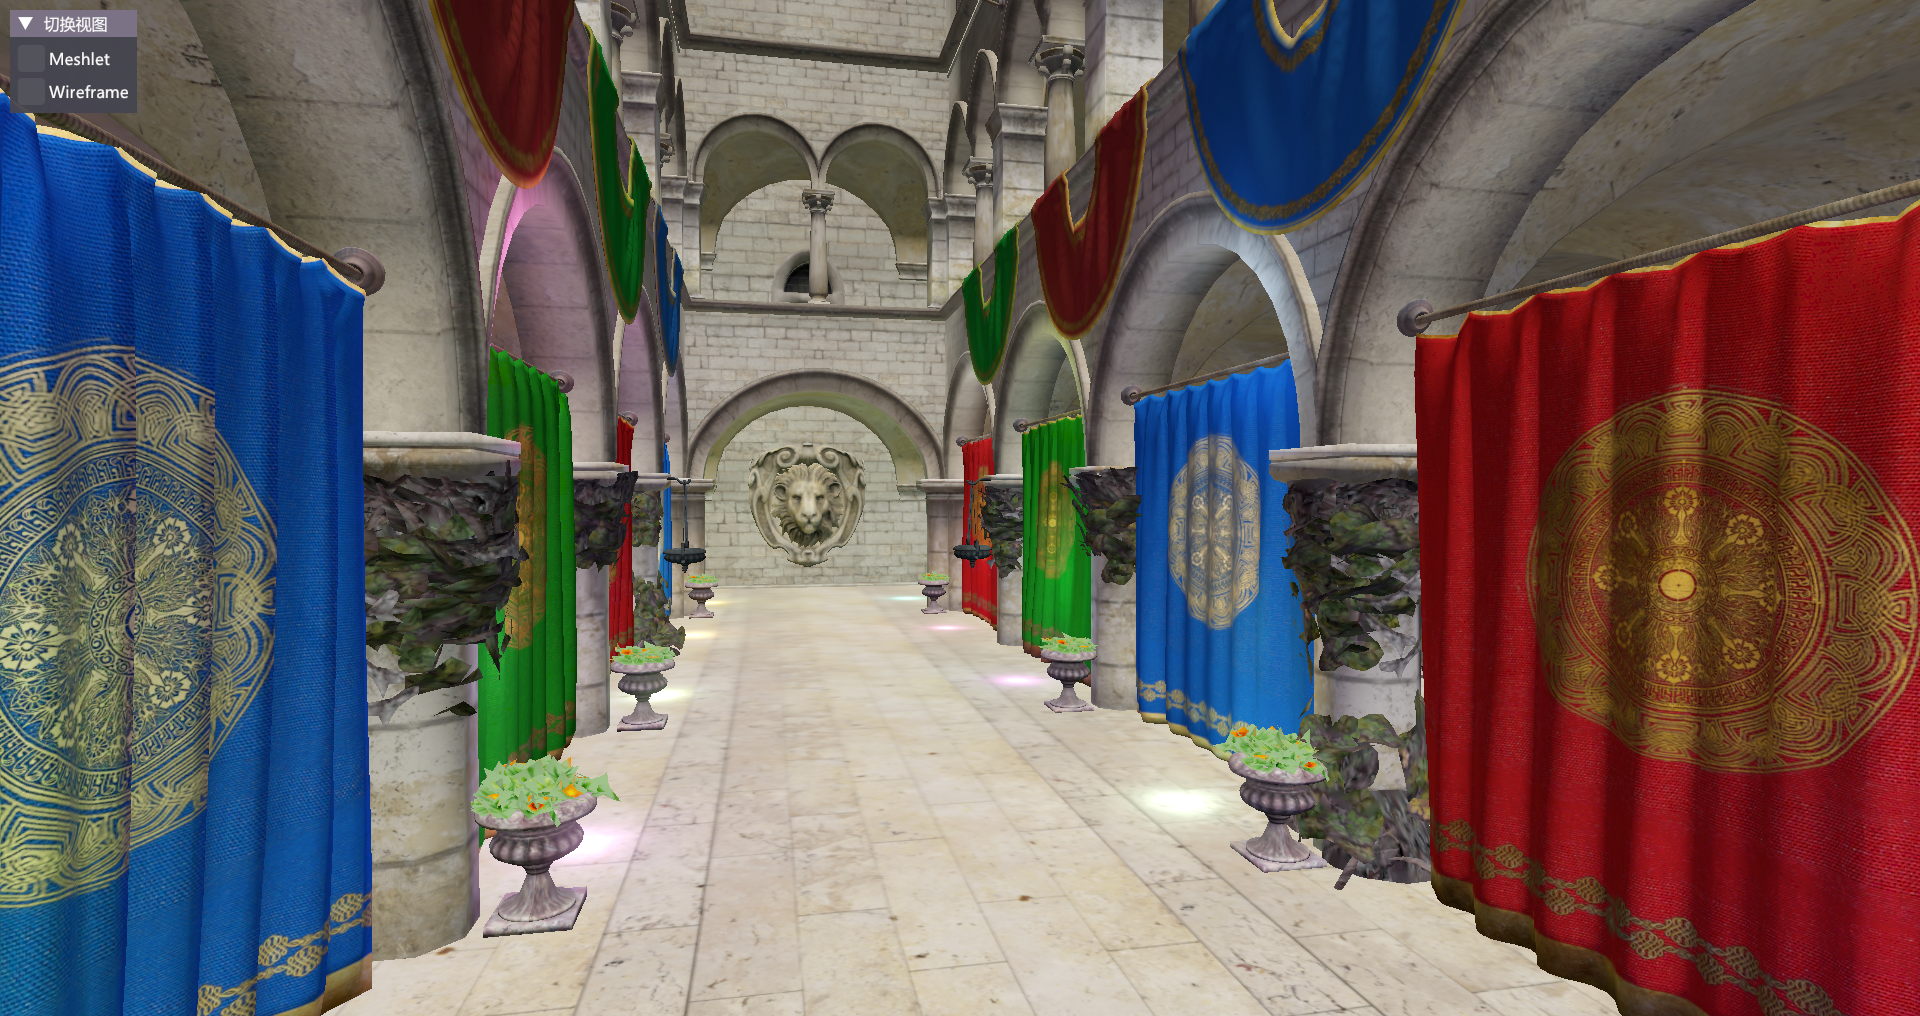
\includegraphics[width=2.9in]{Sponza0.png}
        \caption{不开启 LOD 和流式加载}
    \end{subfigure}%
    \hfill % 确保子图之间有空隙
    % 第二列(中景)
    \begin{subfigure}[b]{0.48\linewidth}
        \centering
        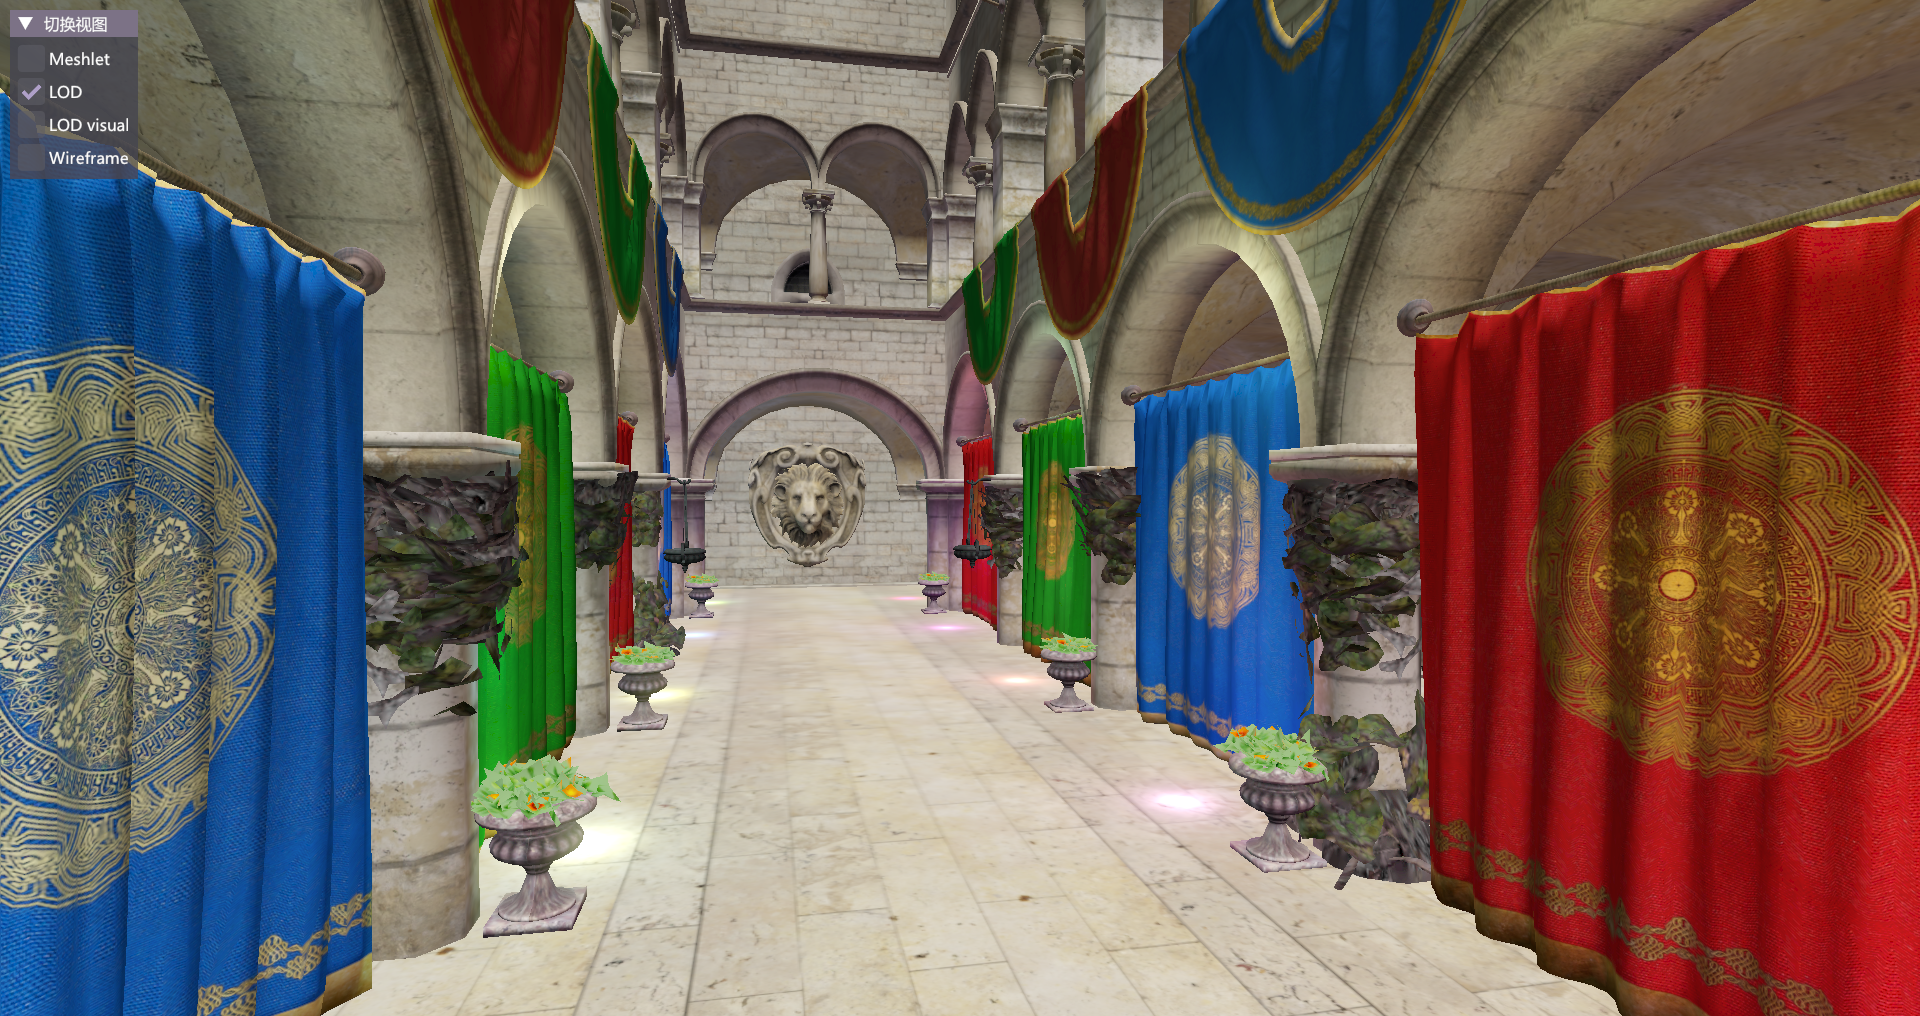
\includegraphics[width=2.9in]{Sponza1.png}
        \caption{开启 LOD 和流式加载}
    \end{subfigure}%
    \caption{Sponza 场景运行效果对比图}
    \vspace{-0.2cm}
    \label{fig:Sponza fig}
\end{figure*}

\begin{table}[H]
    \caption{\label{tab:Factory data}Factory 场景运行参数}
    \begin{tabularx}{\linewidth}{|X<{\centering}|X<{\centering}|X<{\centering}|X<{\centering}|X<{\centering}|}
        \hline
        ~ & 预处理时间 & 显存占用 & GPU 时间 & 帧时间 \\ \hline
        不开启 LOD 和流式加载 & 61s & 5.2GB & 230.3ms & 231.9ms \\ \hline
        开启 LOD 和流式加载 & 1480s & 5.1GB & 38.2ms & 38.5ms \\ \hline
    \end{tabularx}
\end{table}

\begin{figure*}[htbp]
    \centering
    % 第一列(远景)
    \begin{subfigure}[b]{0.48\linewidth}
        \centering
        \includegraphics[width=2.9in]{Factory0.jpg}
        \caption{不开启 LOD 和流式加载}
    \end{subfigure}%
    \hfill % 确保子图之间有空隙
    % 第二列(中景)
    \begin{subfigure}[b]{0.48\linewidth}
        \centering
        \includegraphics[width=2.9in]{Factory1.jpg}
        \caption{开启 LOD 和流式加载}
    \end{subfigure}%
    \caption{Factory 场景运行效果对比图}
    \vspace{-0.2cm}
    \label{fig:Factory fig}
\end{figure*}

从实验结果来看,对于简单场景(如 Sponza),LOD 与流式加载带来的性能收益较为有限;而在复杂工业场景(如 Factory)中,这些优化措施显著提升了渲染性能。帧率从不足 5 FPS 提升至约 25 FPS,实现了接近 5 倍的加速,基本满足实时交互需求。同时可见,开启流式加载后 GPU 时间与整体帧时间相近,说明虽然存在 CPU 与 GPU 之间的数据交互,但并未造成明显的 CPU 负担,系统整体处于良好的负载均衡状态。

不过,优化效果仍存在一些问题。如\autoref{fig:Factory fig}所示,开启 LOD 后画面出现明显走样,初步分析是由于 LOD 生成过程中顶点合并导致法向量精度下降,从而引起光照计算偏差。后续需进一步改进法向量处理策略,以提升画面质量。

与此同时,启用 LOD 与流式加载功能后,预处理耗时显著增加,对于千万级多边形的模型,预处理时间可达 25 分钟左右。为避免用户在每次使用引擎时都重复执行该过程,本项目将预处理后的数据通过可持久化存储保存至磁盘\cite{cereal}。此举不仅显著提升了系统的启动效率,还保证了预处理结果的一致性,方便在后续运行中快速加载和复用。

\subsection{工作总结}

综上所述,本项目在深入理解 Nanite 核心思想的基础上,结合 Vulkan 这一现代图形 API 和现有引擎架构,成功实现了基于簇的 GPU 驱动渲染管线。通过引入 LOD 管理与流式加载机制,系统能够高效导入并实时渲染高复杂度的工业场景,尤其在场景数据体量远超显存容量的情况下,借助流式加载与智能资源调度,依然可实现稳定渲染。在 LOD 技术支持下,系统能够根据视角与物体间距动态调整渲染精度,兼顾画质与性能,显著提升了整体渲染效率。与传统 CPU 驱动渲染管线相比,本项目在大规模工业场景中的性能提升最高可达约 5 倍。

总体而言,本项目为大规模高精度工业数据的实时可视化提供了切实可行的技术路径,并为今后在该领域的进一步研究与应用奠定了坚实基础。

\subsection{未来展望}

尽管本项目在大规模工业场景的实时渲染方面已取得初步成果,但距离实际工程应用仍存在一定差距。未来的改进方向主要包括:

\begin{itemize}
    \item \textbf{增加阴影支持}:当前渲染管线尚未实现阴影效果,缺乏空间深度感。可参考虚幻引擎中的虚拟阴影贴图(Virtual Shadow Map, VSM)方案\cite{VSM},集成高效的实时阴影算法,以提升画面真实感与视觉层次。

    \item \textbf{实现高效的遮挡剔除}:当前管线缺乏高效的遮挡剔除(Occlusion Culling)机制。未来可引入遮挡查询技术(如基于视锥体剔除或 GPU 加速的遮挡测试)来减少不必要的渲染工作,进一步提高性能\cite{coorg1997};

    \item \textbf{支持多材质系统}:当前渲染管线尚未支持多材质系统。未来可以通过实现延迟渲染材质(Deferred Material)来支持多个材质的同时渲染\cite{burns2013},从而提升复杂场景的渲染效果和效率;

    \item \textbf{实现场景数据编码与解码}:通过对场景数据进行高效编码并在 GPU 上解码,可以显著降低显存和主内存占用。同时,数据压缩与编码还能够减少磁盘空间的使用,提高场景数据的加载速度。这将优化显存、内存和存储的资源管理,提升渲染性能和系统响应速度\cite{Mlakar2024}。
\end{itemize}

上述改进将进一步提升本项目在工业级大规模场景中的实时渲染能力和视觉表现力,为其在工程可视化、数字孪生等更广泛的实际应用中奠定技术基础。